\documentclass{standalone}
\usepackage[dvipsnames]{xcolor}
\usepackage{tikz}
\usepackage{fontspec}
\begin{document}
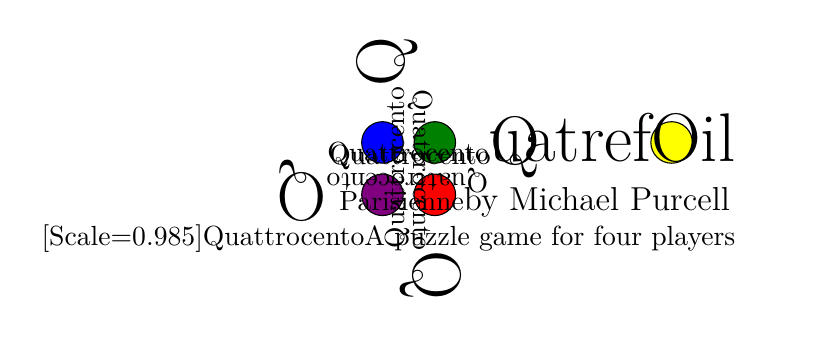
\begin{tikzpicture}
%	\node[circle, fill=Yellow, draw, minimum size=11] () at (-0.915,-0.125) {};
%	\node[circle, fill=Red, draw, minimum size=15] () at (-3.84-0.675,0) {};
%	\node[circle, fill=Green, draw, minimum size=15] () at (-3.84,0.025) {};
%	\node[circle, fill=Yellow, draw, minimum size=15] () at (-3.84-0.675,-0.675) {};
%	\node[circle, fill=Blue, draw, minimum size=15] () at (-3.84,-0.675) {};

	\node[circle, fill=Yellow, draw, minimum size=15] () at (-0.9925,-0.035) {};
	\node[circle, fill=Green, draw, minimum size=15] () at (-4,-0.035) {};
	\node[circle, fill=Red, draw, minimum size=15] () at (-4,-0.7) {};
	\node[circle, fill=Purple, draw, minimum size=15] () at (-4.665, -0.7) {};
	\node[circle, fill=Blue, draw, minimum size=15] () at (-4.665,-0.035) {};



	\node[anchor=east, inner sep=5pt] () at (0,0) {{\setmainfont{Quattrocento}\Huge uatrefOil}};
	\node[anchor=east, inner sep=7pt] () at (0,-0.8) {{\setmainfont{Parisienne}\large by Michael Purcell}};
%		\node[anchor=east, inner sep=7pt] () at (0,-0.75) {{\setmainfont{Parisienne}\large A puzzle game}};
		\node[anchor=east, inner sep=5pt] () at (0,-1.25) {{\setmainfont[Scale=0.985]{Quattrocento}A puzzle game for four players}};

	\node[rotate=0] () at (-4, -0.09) {{\setmainfont{Quattrocento}\Huge Q}};
	\node[rotate=-90] () at (-4.055, -0.7) {{\setmainfont{Quattrocento}\Huge Q}};
	\node[rotate=180] () at (-4.665, -0.645) {{\setmainfont{Quattrocento}\Huge Q}};
	\node[rotate=90] () at (-4.610, -0.035) {{\setmainfont{Quattrocento}\Huge Q}};

	

%	\node[circle, fill=Yellow, draw, minimum size=2.5, inner sep = 0pt] () at (-0.545,0.28) {};

\path (-5.5,-2.375) to (0.5,1.275);
\end{tikzpicture}
\end{document}